\section{The Method of Maximum Likelihood}%9.7
Recall, the likelihood function is simply the joint pdf with the interpretation that a parameter(s) is unknown.
$$Y_1 \sim \text{ via } f(y \mid \theta)$$
$Y_i$'s are iid random sample.

\nl If $\theta$ is known, the joint pdf is
\begin{align}
    \setGreen \underbrace{\setBlack f(\thru{y})}_{\text{domain } f\; \subseteq\; \R^n}\setBlack  &= \color{red} \underbrace{\setBlack f_1(y_1) \cdot f_2(y_2) \cdots f_n(y_n)}_{\text{product of marginals}} & \text{ by independence}\notag\\
    &= f(y_1) \cdot f(y_2) \cdots f(y_n) & \text{by i.i.d.}\notag\\
    &= \prod_{i=1}^n f(y_i)\notag
\end{align}
If $\theta$ unknown, we emphasize this via the \bu{likelihood function}.
%make left underbrace green, right red
$$\setGreen \underbrace{ \setBlack L(\thru{Y} \mid \theta) }_{\text{domain } L\; \subseteq\; \R^{n+1}} \setBlack = \color{red} \underbrace{\setBlack f(y_1 \mid \theta) \cdot f(y_2 \mid \theta) \times \cdots\times f(y_n \mid \theta)}_{\text{really the same}}$$

\disc The reason this is called a \say{likelihood} function. Given a set of observations $Y_i$, what is the most likely value of $\theta$. 

\nl \underline{Fix} $(\thru{Y})$, $L$ at this number is a 1 variable function in terms of $\theta$.
\begin{center}
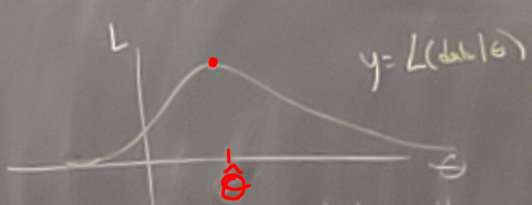
\includegraphics[width=4in]{L fn.png}
\end{center}
\nl Given this data set, what is the most likely value that $\theta$ takes? That would be $\theta$ corresponding to the largest value of pdf $\prod_i^n f(y_i \mid \theta)$.

\nl How do we find the largest? (\color{red}Optimize with respect to $\theta$\color{black}). That is, set $\displaystyle \pdv{L}{\theta} = 0$ solve and verify.

\defn The solution to $L_{\theta} = 0$ defines an estimator $\that$ of $\theta$, called the maximum likelihood estimator (MLE).

\nl \textit{Remark:} In computations, verify the critical point \textit{is} a maximum.

\newpage\noindent\example* $X \sim \operatorname{Bern}(p) = \operatorname{Binom}(1,p)$

\nl Given $\thru{X}$ an iid sample.
\begin{align}
    L(\thru{X} \mid p) &= p^{X_1}(1-p)^{1-X_1} \cdots p^{X_n}(1-p)^{1-X_n} \notag\\
    &= p^S(1-p)^{n-S}, \qquad S := \sum X_i\notag
\end{align}
Then,
\begin{align}
    \pdv{L}{p} &= Sp^{S-1}(1-p)^{n-S} + p^S (n-s)(1-p)^{n-S-1} (-1)\notag\\
    &= p^{S-1}(1-p)^{n-S-1}\brac{S(1-p)-p(n-S)}\notag
\end{align}
And $\displaystyle \pdv{L}{p} = 0$ when 
\begin{align}
    S - Sp - pn + Sp &= 0\notag\\
    S-pn &= 0\notag\\
    p &= \frac{S}{n} = \Xbar\notag
\end{align}
Is this a max? Yes, use the $1^{\text{st}}$ derivitive test: $\displaystyle \pdv{L}{p} = p^{S-1}(1-p)^{n-S-1} \brac{S-pn}.$

\nl If $p < \dfrac{S}{n}$, then $\;\displaystyle \pdv{L}{p} > 0.\;$

\nl If $p > \dfrac{S}{n}$, then $\;\displaystyle \pdv{L}{p} < 0$

\nl Therefore $\Xbar$ is an MLE for $p$. 

\disc The log-likelihood function.
$$L(\vec{X} \mid \theta) = \prod_{i=1}^n f(X_i \mid \theta)$$
Always an $n$-product. Depending on $f$, computing $\pdv{L}{\theta}$ can be difficult.

\nl Since $f(X_i \mid \theta) > 0$ and we have a function whose existance is to turn products into sums$\dots$

\defn The log-likelihood function:
$$\ln L(\vec{X} \mid \theta)$$
Claim: The MLE of $L(\vec{X} \mid \theta)$ also maximizes $\ln L(\vec{X} \mid \theta)$

\nl Reason:
$$\pdv{}{\theta}\pars{\ln L(\vec{X} \mid \theta)} = \frac{\displaystyle \pdv{L}{\theta} \pars{\vec{X}\mid \theta}}{L(\vec{X} \mid \theta)} = 0 \quad \iff \quad \; \pdv{}{\theta}\pars{L(\vec{X} \mid \theta)} = 0$$

\example The last one again\dots
$$L(\thru{X}\mid p) = p^S (1-p)^{n-S}, \quad S := \sum X_i$$
$$\ln L(\vec{x} \mid p) = S\ln p + (n-S)\ln (1-p)$$
$$\pdv{}{p}\pars{\ln L} = \frac{S}{p} + (n-s) \cdot \frac{-1}{1-p}$$
\begin{align}
    \pdv{}{p}\pars{\ln L} = 0 \quad \Longleftrightarrow& \quad S(1-p) + (n-S)(-p) = 0\notag\\
    \Longleftrightarrow& \quad S - Sp - np + Sp = 0\notag\\
    \Longleftrightarrow& \quad p = \frac{S}{n}\notag
\end{align}

\nnl \textbf{Topic: } More population parameters.

\nl This idea scales. If $f$ depends upon $k$ unknowns $\theta_1, \dots, \theta_k$, then define
$$L(\thru{X} \mid \theta_1, \dots, \theta_k) = \prod_{i=1}^n f(x_i \mid \theta_1, \dots, \theta_k)$$
Optimizing this is a calculus problem.

\remark* We could have also extended the idea of the Factorization Theorem the same way with sufficient statistics to get 
$$L(\thru{x} \mid \theta_1, \dots, \theta_k) = \blue{g(S_1, \dots, S_k, \theta_1, \dots, \theta_k) }\cdot \red{h(\thru{x})}$$

\example* Let $\thru{X}$ be an iid from $\normalDist*$ with both parameters unknown. Find the MLE for $\mu$ and $\sigma^2$.

\nl For ease of computation, $N(\mu, \theta)$ such that $\theta := \sigma^2$.
$$L(\thru{x} \mid \mu_1 = \theta) = \prod_{i=1}^n \over{\sqrt{2\pi\theta}}\exp\brac{-\dfrac{(X_i-\mu)^2}{2\theta}}$$
Fixing $\vec{x}$, we consider $L_{\vec{x}}(\mu,\;\theta)$\dots. I have no intentions of $\nabla L_{\vec{x}}$ under a product sign\dots
\begin{align*}
    \ln L &= \sum_{i=1}^n \pars{\ln(\over{\sqrt{2\pi\theta}}) + \dfrac{-(X_i-\mu)^2}{2\theta}}\\
    &= - \over{2} \ln (2\pi\theta)n - \over{2\theta} \sum_{i=1}^n (X_i-\mu)^2
\end{align*}
\begin{align*}
    \pdv{}{\mu}\pars{\ln L} &= 0 - \over{2\theta} \sum_{i=1}^n 2(X_i-\mu)(-1)\\
    &= \over{\theta} \sum (X_i-\mu)\\
    &= 0 \quad \text{when} \quad \textstyle \sum X_i - n\mu = 0 \rightarrow \widehat{\mu} = \Xbar 
\end{align*}
$$\text{i.e. } \mu = \dfrac{1}{n}\sum X_i = \Xbar$$

\begin{align*}
    \pdv{}{\theta}\pars{\ln L} &= -\frac{n}{2} \cdot \frac{2\pi}{2\pi\theta} + \over{2\theta^2} \sum_{i=1}^n(X_i-\mu)^2\\
    &= -\frac{n}{2\theta} + \over{2\theta^2} \sum_{i=1}^n(X_i-\mu)^2\\
    &= 0 \quad \text{At our potential critical point } \mu = \Xbar\\
    &\iff -n\theta + \sum_{i=1}^n(X_i-\Xbar)^2 = 0\\
    \text{or } & \that = \over{n}\sum_{i=1}^n(X_i-\Xbar)^2\\
    & \red{\text{our old biased estimator for } \sigma^2}
\end{align*}
Is this a max? We need to construct the Hessian Matrix\dots
\begin{align*}
    H &= \bmat{\ln L_{\mu\mu}}{\ln L_{\mu\theta}}{\ln L_{\theta\mu}}{\ln L_{\theta\theta}}\\
    &= \bmat{-\dfrac{n}{\that}}{-\dfrac{\sum X_i - n\mu }{\that^2}}{-\dfrac{\sum X_i - n\mu }{\that^2}}{\dfrac{n}{2\that^2}-\dfrac{1}{\that^3} \sum(X_i-\mu)^2}\\
    \text{At } (\widehat{\mu},\;\that) \\
    H(\mu, \theta) &= \bmat{-\dfrac{n}{\that}}{0}{0}{\dfrac{n}{2\that^2}-\dfrac{1}{\that^3} \sum(X_i-\mu)^2}
\end{align*}
For a maximum, by the $2^{\text{nd}}$ derivitive test, we need $(\ln L)_{\mu\mu} = -\dfrac{n}{\that} < 0$, \hspace{.1cm} \red{which it is! } And $\det H > 0$.

\nl Note, $\displaystyle (\ln L)_{\theta\theta} = \dfrac{\that n - 2 \sum(X_i - \Xbar)^2}{2 \that^3}$.

\nl But $n\that = \sum (X_i - \Xbar)^2$, so $\displaystyle (\ln L)_{\theta\theta} = \dfrac{\that n - 2 \that n}{2 \that^3} = - \frac{n}{2\that^2} \;\red{ < 0}$.

\nl So $\displaystyle \det H = \dfrac{-n}{\that} \cdot \dfrac{-n}{2\that^2} = \dfrac{n^2}{2\that^3}\;\red{ > 0 }$. Hence $(\Xbar,\, \that)$ is the location of a MLE by the 2nd derivitive test.

\disc Why MLEs? Because they have nice properties.
\begin{enumerate}[label=\textcircled{\raisebox{-1pt}{\arabic*}}]
    \item If $U$ is a sufficient statistic of $\theta$, then the MLE \red{is} a function of $U$.
    
    \nl Reason: If $U$ is sufficient, then $L(\vec{x} \mid \theta)$ is factorable:
    $$L(\thru{x} \mid \theta_1, \dots, \theta_k) = g(U, \theta) \cdot h(\thru{x})$$
    This $\displaystyle \pdv{L}{\theta} = \pdv{g}{\theta} \cdot h(\vec{x})$ 
    $$\text{i.e. }\; \underbrace{ \pdv{L}{\theta} = 0 }_{  
        \substack{ \text{sol'n to this is} \\ \that \text{ (the MLE)} }
    } \iff \underbrace{\pdv{g}{\theta} = 0}_{
        \substack{\text{sol'n to this is} \\ \that \text{ a function of } U}
    }$$

    \item The invariance properties of the MLE.
    
    \nl Suppose we want to estimate a function of the parameter (say $t(\theta)$). If $t$ is a one-to-one (injective) function (i.e. invertible), the MLE of $t(\theta)$ will be simply $t(\that)$, where $\that$ is the MLE of $\theta$.

    \nl Reason: Let $t(\theta)$ be injective. Assume $\that$ the MLE of $\theta$ $t(\theta)$ invertible $\implies$ $\Psi = t(\that)$ and $t^{-1}(\Psi) = \theta$

    \nl Then $L(\vec{x} \mid \theta)$ is maximized at $\theta = \that$. Then $L(\vec{x} \mid t^{-1}(\Psi))$ is maximized at the same $\that$. Hence $t^{-1}(\Psi) = \that$ or $\Psihat = t(\that)$.

    \example (\#1) Show $\Xbar$ is MLE for $\lambda$ when $X \sim \operatorname{Pois}(\lambda)$. 

    \nl In showing $S := \sum X_i$ is sufficient, we had factored the likelihood function 
    $$L(\vec{x} \mid \lambda) = \green{\underbrace{\setBlack e^{-n \lambda}\lambda^S}_{g(S,\;\lambda)}}  \cdot \over{x_1! \cdot x_2! \cdots x_n!}$$
    To find the MLE $\displaystyle \pdv{L}{\lambda} = 0$ when $\displaystyle \pdv{g}{\lambda} = 0$.
    \begin{align*}
        \pdv{g}{\lambda} &= -ne^{n\lambda} \lambda^S + e^{-n\lambda} s\lambda^{S-1}\\
        &= e^{-n\lambda}\lambda^{S-1}\bigbrac{-n\lambda + S}\\
        &= 0\\
        &\implies \lambda = \frac{S}{n} \hspace{1in} \text{i.e. } \widehat{\lambda} = \xbar
    \end{align*}
    As before, can show a max by the 1st derivitive test.

    \example Lots of bits together
    
    \nl We have shown that $\chi^2 \sim \operatorname{Pois}(\lambda)$ with $S = \sum x_i$ is a sufficient statistic for $\lambda$. And we just showed that $\that = \xbar$ is MLE for $\lambda$. 

    \nl Hence, by the Rao-Blackwell Theorem, $\E{\Xbar \mid S} = \Xbar$, then $\Xbar$ is an MVUE for $\lambda$. At the end of RBT, via
    $$w = 
    \left\{ \begin{array}{cc}
            1 & \hspace{5mm} x_1 = 0 \\
            0 & \hspace{5mm} x_1 \neq 0
            \end{array} \right. (w \text{ unbiased for } e^{-\lambda})$$
            Combining $w$ with $S$ we get the MVUE $\Psihat = \pfrac*{n-1}{n}^S = \pfrac*{n-1}{n}^{n\Xbar}$ for $e^{-\lambda}$. \red{(also $\Var*{\Psihat} < \Var*{w} $)} \hspace{1mm} by RBT.

            \nl Now, since $\Xbar$ is MLE for $\lambda$, by the invariance properties of MLE,
            $$\theta^* = e^{-\Xbar} \; \text{ is MLE for } e^{-\lambda}.$$
            Reason: $g(x) = e^-x$ is clearly injective on $\R$.

            \nl Moreover, by RBT $\Var*{\Psihat} < \Var{e^{-\Xbar}}$. And we have a conjecture that $e^{-\Xbar}$ is actually biased.

            \nl While $e^{-\Xbar}$ is the \say{natural} estimator for $e^{-\lambda}$, the RBT says $\Psihat = \displaystyle \pfrac*{n-1}{n}^{n\Xbar}$ is \red{\say{better}} \hspace{0.5mm} as $\Psihat$ \underline{is} unbiased and $\Var*{\Psihat} < \Var*{\theta^*}$.

            \nl \red{Q: Can we show this directly?}
            \\Maybe. \red{If $\theta^*$ is unbiased\dots}
            $$\Var*{\Psihat} < \Var*{\theta^*} \leftrightsquigarrow \Eb{(\Psihat)^2} < \Eb{(\theta^*)^2}$$
            FACT: $\displaystyle \limn \pfrac*{n-1}{n}^n = \limn \pars{1-\over*{n}}^n = e^{-1}$. (This is via Calc I application of L'Hopitals)

            \nl Moreover, via the same $\ln$ technique, it can be shown that $f(x) = \pfrac*{x-1}{x}^x$ is increasing on $x \geq 2$ (see addendum). Hence,
            \begin{align*}
                & \pfrac{n-1}{n}^n < e^{-1}\\
                \implies & \pfrac{n-1}{n}^{2n} < e^{-2}\\
                \implies & \pfrac{n-1}{n}^{2n\Xbar} < e^{-2\Xbar}\\
                \implies & \pars{\pfrac{n-1}{n}^{n\Xbar}}^2 < {e^{-\Xbar}}^2\\
                \implies & \E{\Psihat^2} < \E{(\theta^*)^2}\\
                \implies & \Var{\Psihat} < \Var{\theta^*}\\
                & \red{\text{(if } \theta^* \text{ is unbiased)}}
            \end{align*}

            \newpage\noindent \textbf{Addendum:}
            
            \nl Claim: $f(x) = \displaystyle \pfrac*{x-1}{x}^x$ is increasing on $x \geq 2$.

            \nl Reason:
            \begin{align*}
                \ln f &= x \ln (x-1) - x \ln x\\
                \frac{f'}{f} &= \ln (x-1) + \frac{x}{x-1} - \ln x - 1\\
                &= \ln \pfrac{x-1}{x} + \over{x-1}\\
                f'(x) = 0 \implies& \ln \pfrac{x-1}{x} + \over{x-1} = 0
            \end{align*}
            But this does not happen on $(1, \infty)$. Equivalently, $\displaystyle \ln \pfrac*{x-1}{x}^{1-x} = 1 \implies \dfrac{x-1}{x} = 1$ has no solutions.

            \nl Since $f'(2) = \ln \pfrac*{1}{2} + 1 = 1 - \ln 2 > 0$, we get $f'(x) > 0$ on $(1, \infty)$.
            
\end{enumerate}